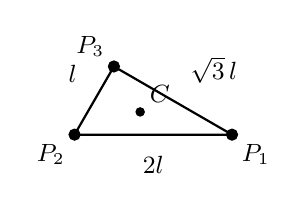
\begin{tikzpicture}[scale=1, font=\small]
  % Problem 5-15: Three points P1, P2, P3 forming a triangle
  % P1-P2 distance = 2l, P2-P3 = l, P1-P3 = sqrt(3)*l
  % This is a right triangle: P3 is the right angle vertex

  % Place P2 at origin, P1 at (2l, 0)
  \coordinate (P1) at (2, 0);
  \coordinate (P2) at (0, 0);
  \coordinate (P3) at (1.5, 0.866); % Using law of cosines

  % Actually let me recalculate. P1-P2=2l, P2-P3=l, P1-P3=sqrt(3)l
  % P2 at origin, P1 at (2,0)
  % P3 distance l from P2, sqrt(3)*l from P1
  % cos(angle at P2) = (4+1-3)/(2*2*1) = 2/4 = 0.5 => angle = 60 deg
  \coordinate (P2) at (0, 0);
  \coordinate (P1) at (2, 0);
  \coordinate (P3) at ({cos(60)},{sin(60)}); % = (0.5, 0.866)

  % Draw triangle
  \draw[thick] (P1) -- (P2) -- (P3) -- cycle;

  % Points
  \filldraw (P1) circle (2pt) node[below right] {$P_1$};
  \filldraw (P2) circle (2pt) node[below left] {$P_2$};
  \filldraw (P3) circle (2pt) node[above left] {$P_3$};

  % Center of mass
  \coordinate (C) at ({(2+0+0.5)/3},{(0+0+0.866)/3});
  \filldraw[fill=black] (C) circle (1.5pt) node[above right] {$C$};

  % Distance labels
  \node[below] at (1, -0.15) {$2l$};
  \node[above left] at ({(0+0.5)/2-0.1},{(0+0.866)/2+0.1}) {$l$};
  \node[above right] at ({(2+0.5)/2+0.1},{(0+0.866)/2+0.1}) {$\sqrt{3}\,l$};
\end{tikzpicture}
